
\section{Complexity of users' searches over time}

\subsection{Definitions}

The \textbf{complexity} of a search query is the number of fields that aren't \emph{course number} or \emph{department} that it spans. The accepted fields are shown in the following table:

\singlespacing
\begin{center}
\begin{table}[H]
  \centering
  \begin{tabular}{ lllll }

    \hline

    description
    & title
    & credits
    & crosslisted
    & CRN
    \\

    
    instructor
    & year
    & term
    & upper-level writing
    & random
    \\

    \hline

  \end{tabular}
  \vspace{10pt}
  \caption{``Complex'' search fields (omits only \emph{number} and \emph{department})}
  \label{fig:sc-fields}
\end{table}
\end{center}
\doublespacing

\noindent We can compute the number of searches it takes a user to reach a new highest search complexity record since the previous record. See Table \ref{fig:sc-example} for an illustrative example.

A user's \textbf{first increase in search complexity} is defined as the number of searches a user made before searching with complexity greater than zero. If a user's first search has complexity 1, the user's \emph{first increase} is 0.

A user's \textbf{second increase in search complexity} is defined as the number of searches a user made before searching with complexity greater than their \emph{first increase}'s search complexity.

It is possible that a user has neither metric, both metrics, or only a \emph{first increase} metric.

{\renewcommand{\arraystretch}{2.0}
\singlespacing
\begin{center}
\begin{table}[H]
  \centering
  \begin{tabular}{ r | c c c | l }

    Query no.
    & Search query
    &
    & Complexity
    & Searches till increase \\

    \hline

    \#1
    & ``{\tt CSC}''
    & \rightarrow
    & 0
    & \hspace{55pt} ---
    \\

    \#2
    & ``{\tt MTH 165}''
    & \rightarrow
    & 0
    & \hspace{55pt} ---
    \\

    \#3
    & ``{\tt csc taught by guo}''
    & \rightarrow
    & 1
    & $3-1=\textbf{2}$ \hspace{2pt} \emph{(first increase)}
    \\

    \#4
    & ``{\tt random mur 1-2 credits}''
    & \rightarrow
    & 2
    & $4-3=\textbf{1}$ \hspace{2pt} \emph{(second increase)}
    \\

  \end{tabular}
  \vspace{10pt}
  \caption{Illustration of computing the number of searches before a complexity increase}
  \label{fig:sc-example}
\end{table}
\end{center}
\doublespacing


\subsection{Motivation}

The purpose of this metric is to determine the usability and learning curve of SkedgeQL. The two ways Skedge currently offers to teach users about its query language are

\begin{enumerate}
  \item  by providing a table of example queries whenever the user clicks inside the search field from the Skedge homepage (see Figure \ref{fig:sk-search2}), and

  \item  from embedded links on the site making searches with high complexity and implicitly demonstrating them to users by using the same input field they use to submit searches.\footnote{Clicking on an instructor's name, for instance, makes the advanced search ``for the user.'' Another example is clicking on a course box in the side schedule, which searches for that course code along with its term and year (e.g. ``{\tt CSC 171 Fall 2016}'').

  Other possibilities include linking the credits field of each course to a credits search, the CRN field of a section to a CRN search, the ``{\tt W}'' part of the course code to an upper-level writing search, having a crosslisted course link search the crosslisting of the two departments (instead of directly link to the crosslisted course), or a ``feeling lucky?'' button for a search with ``{\tt random}''.}
\end{enumerate}

\begin{figure}[H]
  \centering
  \fbox{
    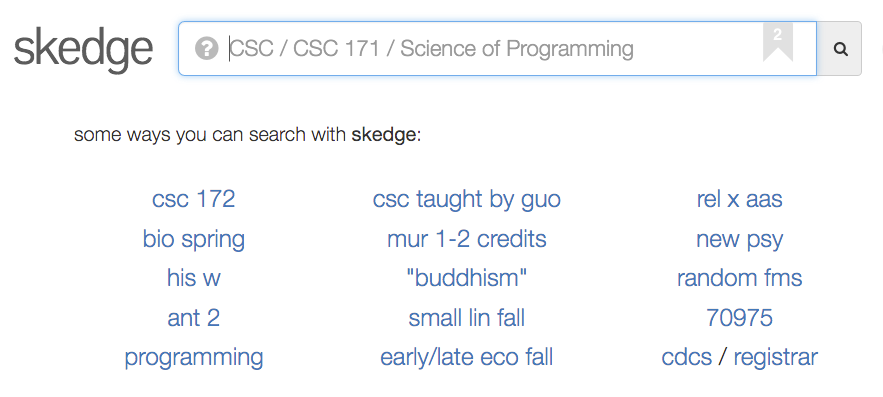
\includegraphics[width=0.65\textwidth]{images/skedge/search}
  }
  \caption{Examples of SkedgeQL} \label{fig:sk-search2}
\end{figure}

\noindent The latter method is, of course, much preferred to the former as it teaches without requiring concerted effort on the part of the user to study and learn the query language, and mostly likely remains more memorable and intuitive as a result.

A \emph{high} percentage of users with \emph{first increase} and \emph{second increase} metrics, with \emph{low} mean and median values for those increases would be desirable. This would strongly indicate the effect of teaching method \#2 because the factor in teaching users about the query language would simply be time (besides the case of users becoming curious about advanced search types and looking them up explicitly, which is difficult to account for because the query example box is shown to all users fairly regularly).

\subsection{Trends}

\subsubsection{Analysis of users with search complexity increases}

\begin{figure}[H]
  \centering
  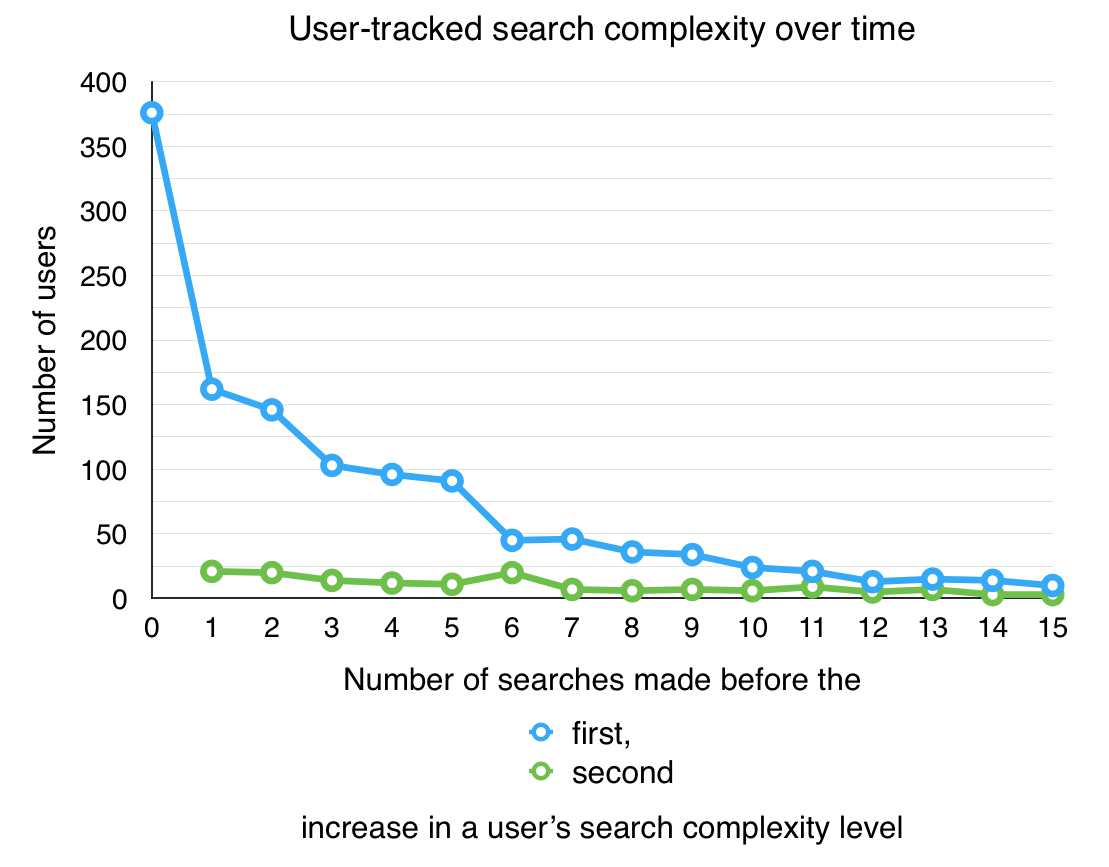
\includegraphics[width=0.9\textwidth]{images/graph/search_dt}
  
  \caption{User-tracked search complexity over time}
  \label{fig:sc-graph}
\end{figure}

The blue line in Figure \ref{fig:sc-graph} plots the number of users that had their \emph{first increase} in search complexity per search index (searches \#16--\#25 represent 47 users, and 26+ searches represents only 29 users). The green line plots the number of users for a \emph{second increase} at the given search index (searches \#16--\#25 represent 35 users, and 26+ searches represents 32).

The amount of users whose first searches are of nonzero complexity may be surprising. The vast majority of these are \textbf{title} searches however, which \emph{are} included in the ``complex'' field table. This is purposeful---title searches only represent 8\% of all search field uses, as we saw in Figure \ref{fig:searchtypes} of the section before last. Moreover, a user's understanding and/or intuition that the Skedge search field is free-form and can be used for different search fields simultaneously is already a significant conceptualization of SkedgeQL, albeit for a relatively basic search type.

\subsubsection{Users with increases vs. users without increases}

\begin{figure}[H]
  \centering
  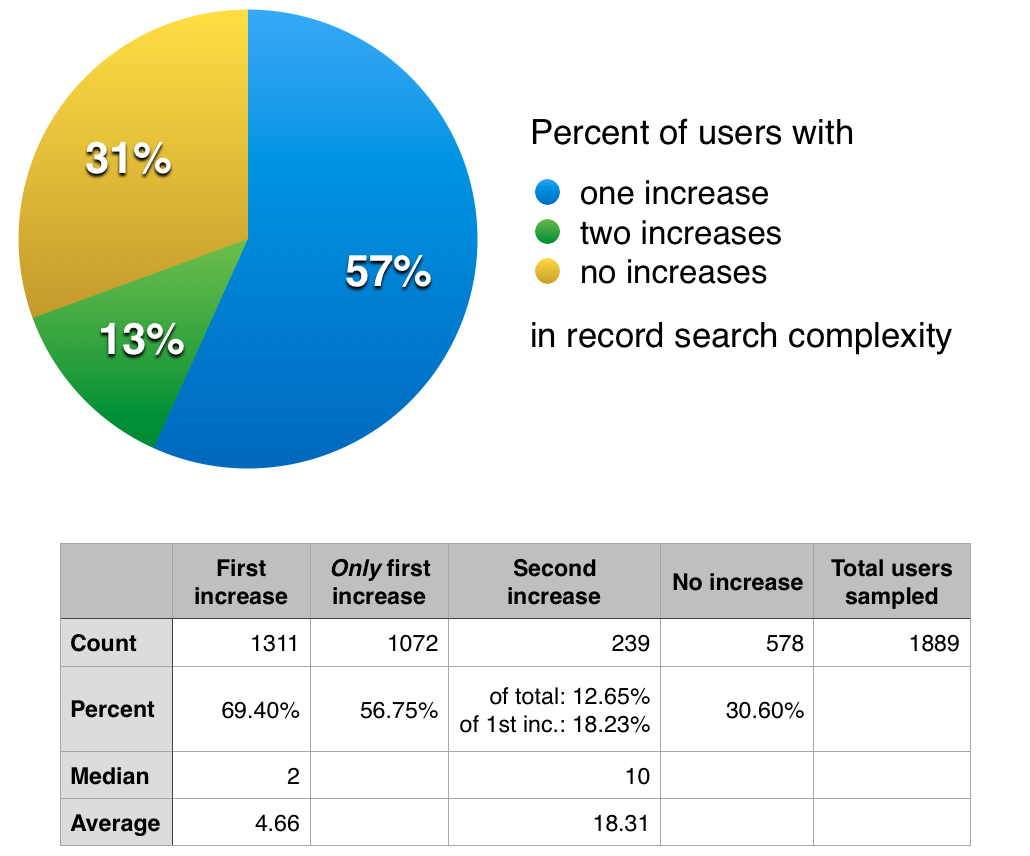
\includegraphics[width=0.9\textwidth]{images/graph/search_dt_pie}

  \caption[Users split by their number of increases in search complexity]{Users with a schedule and more than one search split by their number of increases in search complexity}
  \label{fig:sc-pie}
\end{figure}

\vspace{5pt}

Figure \ref{fig:sc-pie} shows that 69.4\% of Skedge users (\emph{users} here defined as having at least one course bookmarked or added to a schedule, with more than two searches since November 3rd---there are 1889 such users in total) have increased their record search complexity at least once, with a median of 2 searches to do so. Of those users, 18\% of them (12\% of total users) have had a \emph{second} increase in search complexity, with a median of 10 searches to do so. 30\% of users have only searched with the department and course number fields.

I believe this is a strong model for evaluating the friendliness and low learning curve of SkedgeQL, and the results are certainly promising, although further analysis on beginning with nonzero search complexity is needed.